\documentclass{lni}

\IfFileExists{latin1.sty}{\usepackage{latin1}}{\usepackage{isolatin1}}

\usepackage{graphicx}
\usepackage{minitoc}
\usepackage[ngerman]{babel}
\usepackage[ansinew]{inputenc}

% add bibliography to toc
\usepackage[nottoc]{tocbibind}

\begin{document}

\author{
	Martin Helmich, Oliver Erxleben \\ 
	\\ 
	Hochschule Osnabrück \\ 
	Ingenieurswissenschaften und Informatik \\ 
	Informatik - Mobile und Verteilte Anwendungen \\ 
	\\ 
	martin.helmich@hs-osnabrueck.de \\
	oliver.erxleben@hs-osnabrueck.de
}

\title{
\includegraphics[scale=0.75,keepaspectratio]{img/hs_os.png}\linebreak \linebreak OpenMP [Working DRAFT]}

\maketitle

\tableofcontents

\begin{abstract}
Die vorliegende Hausarbeit ist eine gemeinsame Arbeit von Martin Helmich und Oliver Erxleben für das Modul \textit{Parallele und Verteilte Algorithmen} im Wintersemester 2012/13 an der Hochschule Osnabrück. Das Thema der Arbeit ist die Betrachtung von OpenMP zur Parallelisierung von Programmen. \\ 
Die Arbeit gliedert sich in die konzeptionelle Betrachtung und kritische Würdigung von OpenMP und den Vergleich mit der im Modul kennengelernten Programmierbibliothek Threading Building Blocks von Intel. \\
Desweiteren wird die Aufgabe aus Intel`s \textit{Accelerate your Code} - Programmierwettbewerb von Herbst 2012 mittels OpenMP reimplementiert.
\end{abstract}

\pagebreak % new page after toc and abstract

\setcounter{page}{1} % the real document begins here, so set page number to 1
\section{OpenMP}
Open Multi-Processing (kurz: OpenMP) ist eine Programmierschnittstelle für die Sprachen C/C++ und Fortran, welche seit 1997 von unterschiedlichen Hardware- und Compilerherstellern entwickelt wird. Ziel von OpenMP, welches mittlerweile den Versionsstand 3.1 erreicht hat, ist es ein portables und zugleich paralleles Programmiermodell für Shared-Memory-Architekturen\footnote{Shared-Memory-Architektur: } zur Verfügung zu stellen. Es setzt sich aus Compilerdirektiven, Bibliotheksfunktionen und Umgebungsvariablen zusammen. Anders als viele alternative Ansätze zur Parallelisierung von Programmen sind nur wenige Änderungen an sequenziellen Programmen notwendig um parallele Abläufe zu implementieren. Auch die Lesbarkeit des parallelisierten Quelltextes wird im Vergleich zu anderen alternativen Ansätzen stark verbessert. (Vgl. \cite{omp08} Kapitel 1: Einführung)
\\
Compilerdirektiven

\subsection{Merkmale von OpenMP}
Hoher Abstraktionsgrad \\
Portabilität \\
Schrittweise Parallelisierung \\
herstellerübergreifender Standard

\subsection{Ausführungsmodell}
Die parallele Ausführung erfolgt durch Threads auf dem Fork-/Join\footnote{Fork/Join:}-Ausführungsmodell. Zu Beginn eines Programms ist nur ein Thread aktiv, der sog. \textit{Master Thread}. Sobald bei der Programmausführung die Direktive \textit{\#pragma omp parallel \{ ... \} } erreicht wird, gabelt sich die Ausführung in Threads auf. Die erstellten Threads werden als \textit{team of threads} bezeichnet\footnote{Die Implementierung von OpenMP entscheidet über die Art der Threads die erstellt werden. Es könnten Threds auf Basis der PThreads-Bibliothek oder aber auch als vollwertige Shared-Memory-Prozesse umgesetzt sein.}. Für OpenMP, bzw. der Entwicklung mit OpenMP stellen Threads einen Kontrollfluss mit gemeinsamen Adressraum dar.  \\ 
Die schließende geschweifte Klammer ist zudem ein Synchronisationspunkt, andem das team of threads auf alle Teammitglieder wartet. Die Abbildung \ref{Join-Fork-Modell} stellt einen möglichen Ablauf mit OpenMP dar. 

\begin{figure}[h!]
  \centering
    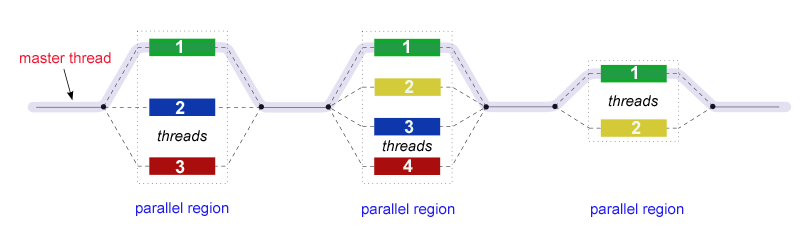
\includegraphics[width=1.0\textwidth]{img/fork_join.png}
    \label{Join-Fork-Modell}
   \caption{Fork-Join-Prinzip}
   \protect{\textit{Entnommen aus OpenMP Tutorial} (\cite{openmptut})}
\end{figure}

\subsection{Parallele Schleifen}
\subsection{Synchronisation}
\subsection{Abschnitte und Aufgaben}

\pagebreak % first part ends

\section{Vergleich mit TBB und anderen?!}

Text Text Text Text Text Text Text Text Text Text Text Text Text Text Text Text Text Text Text Text Text Text Text Text Text Text Text Text Text Text Text Text Text Text Text Text Text Text Text Text Text Text Text Text Text Text Text Text Text Text Text Text Text Text Text Text.

\subsection{Unterkapitelüberschrift}

Text Text Text Text Text Text Text Text Text Text Text Text Text Text Text Text Text Text Text Text Text Text Text Text Text Text Text Text Text Text Text Text Text Text Text Text Text Text.

%\begin{figure}[htb]
%  \begin{center}
%    \includegraphics[width=2cm]{gilogo}
%    \caption{\label{logo}Beschreibung der Abbildung}
%  \end{center}
%\end{figure}

Text Text Text Text Text Text Text Text Text Text Text Text Text Text Text Text Text Text Text Text Text Text Text Text Text Text Text Text Text Text Text Text Text Text Text Text Text Text.

Text mit Fußnote.\footnote{Dies ist eine Fußnote. Text Text Text Text Text Text Text Text Text Text Text Text Text Text Text Text Text Text Text.} Text \cite{Ez99,ABC01} Text Text Text Text Text Text Text Text Text Text Text Text Text Text Text Text Text Text Text Text Text Text Text Text Text Text Text Text  Text Text Text Text Text Text Text Text Text Text Text Text Text Text Text Text Text Text Text Text Text Text Text Text Text Text Text Text Text Text Text Text Text Text Text Text Text Text Text Text Text.

\pagebreak

\bibliography{lib/references}{}
\bibliographystyle{plain}

\newpage

\listoffigures

\listoftables

\section{Anlagen}
\pagenumbering{none}
\setcounter{subsection}{0} %clear counter 
\minitoc

\nomtcpagenumbers % TODO: the dots remain in eternity... 

\subsection{Source Code}

\subsection{Latex Dateien}


% Vor Abgabe raus!!!! 
\subsection{Working Notes}
Links: 
https://computing.llnl.gov/tutorials/openMP/ \\
http://www.people.westminstercollege.edu/faculty/ggagne/fall2012/306/handouts/parallel/index.html \\
http://www.openmp.org/mp-documents/OpenMP3.1.pdf \\

\end{document}
	